\documentclass{article}

\usepackage{amsmath}
\usepackage{graphicx}
\usepackage{epstopdf}
\usepackage{booktabs}
\usepackage{siunitx}
\usepackage{caption}
\usepackage{url}
\usepackage{abstract}
%\usepackage{tikz,pgfplots} % diagrams and data plots

\captionsetup{margin=12pt,font=small,labelfont=bf}

\renewcommand{\abstractname}{}

\setlength{\absleftindent}{30mm}
\setlength{\absrightindent}{30mm}

\newcommand{\figref}[2][\figurename~]{#1\ref{#2}}
\newcommand{\tabref}[2][\tablename~]{#1\ref{#2}}
\newcommand{\secref}[2][Section~]{#1\ref{#2}}


\begin{document}
\title{Nuclear rods: Partial Differential Equations} 
\author{Ben McMurtry}
\date{7th December 2016} 	
\maketitle







\section{Introduction}
\label{sec:introduction}

A spent nuclear fuel rod will continue to decay radioactively, potentially to a significant degree, for many years, depending on the lifetimes of the remaining radioactive elements. The energy released by these decays will heat up the rod and its surroundings.

This report discusses the methods and results of a program created to calculate the temperature around a nuclear waste rod, after any amount of time had passed, using the method outlined in example 5.3.1 (pages 41-44) of: ``Numerical Solutions of Partial Differential Equations'' (2011) by Louise Olsen-Kettle, University of Queensland\cite{Olsen-Kettle}.

The problem is considered in the following way. The nuclear rods give out heat due to radioactive decay, according to (1).

\begin{equation}
\frac{1}{\kappa} \frac{dT}{dt}(r,t) - \nabla^2 T(r,t) = S(r,t)
\end{equation}

where the Source term due to the radioactivity of the rod is given by:

\begin{equation}
S(r,t) = \begin{cases}
      T_{rod}e^{-t/\tau_0} / a^2, & \text{for}\ r\leq a \\
      0, & \text{otherwise}
    \end{cases}
\end{equation}

And for the modelled scenario, parameters were chosen the same as \cite{Olsen-Kettle}: 

\vspace{5mm}

Rod Radius $a = 25$ cm, 

Thermal conductivity $\kappa = 2\times10^7$ cm2/year, 

Initial temperature change due to rod $T_{rod} = 1$ K,

Lifetime of radioactive decaying nuclei $\tau_0 = 100$ years, 
  
Radius bound for solution $r_c = 100$ cm, 

environment temperature $T_E = 300$ K, 

$0 < r < 100$ cm 

$0 < t < 100$ years

Initial temperature $T(r, t = 0) = 300$ K.

\vspace{5mm}

Since the temperature has no $\phi$ dependence. The problem was reduced to a 1D heat equation in $r$ (3). 

\begin{equation}
\frac{1}{\kappa} \frac{dT}{dt} - \frac{d^2T}{dr^2} - \frac{1}{r} \frac{dT}{dr} = S(r,t)
\end{equation}

There is a singularity at r = 0 in the above equation where special care needs to be taken so that the numerical solution is stable. To do this we  use a Neumann boundary condition stating that temperature cannot flow into r = 0: $\frac{dT}{dr}(r = 0, t) = 0$.

We also use a Dirichlet boundary condition at $r = r_c$ to set the temperature far enough away from the rod is equal to the environment temperature: $T(r=r_c) = T_E$.







\section{Method}

This problem was solved using a Backwards Euler method\cite{BEuler}, with finite differences\cite{FiniteDifference}. 

As a result, for the sake of the model, we discretise space and time in the following way: $\Delta r=r_c/(n+1)$, $\Delta t = T_f /m$, $r_j = j\Delta r$, $0 \leq j \leq n + 1$, $t_k = k\Delta t$, $0 \leq k \leq m$. Meaning the equation to solve was now:

\begin{equation}
A\vec{T}^{k+1} = \vec{T}^k + \kappa \Delta t \vec{S}^k + \vec{b} 
\end{equation}

which is of the form A x = b, where A is a tridiagonal matrix involving a gain parameter $s = \kappa \Delta t / \Delta r^2$ The details of getting from (3) to (4), and the form of the matrix A, have been left out here due to their length, but can be found in pages 43-45 of Dr. Olsen-Kettle's work \cite{Olsen-Kettle}.

The program was created using the C language with the help of the GNU software library (GSL) \cite{GSL}. The GSL header files gsl\_vector.h and gsl\_matrix.h contain useful vector and matrix structures and functions, and the header file gsl\_linalg.h has multiple useful functions for solving linear algebra equations involving vectors and matrices.

In the program created, the gsl function gsl\_linalg\_solve\_tridiag is used, which can be used to solve equations of the general N-by-N system A x = b where A is a positive definite, tridiagonal matrix\cite{Linalg}.

The radial positions (excluding r = 0 and r = $r_c$ as found in \cite{Olsen-Kettle}) (calculated as $j \times \Delta r$) were originally going to be stored in a vector, but then it was decided to store them in the 1st column of the Temp matrix which was created for ease of reproducing figure 5.3(b) with gnuplot. The Temp matrix then had another 4 columns of length $n$, which were placed there to accept the Temperature vectors at the times required for the reproduction of figure 5.3(b).

The Temperature vectors of length $n$, were stored in either vector T\_even or T\_odd based on whether the time index $k$ was even or odd for that timestep. Having both T\_even and T\_odd allowed us to keep a store of the previous temperature which was to be used in the b vector.

The tridiagonal matrix A, for the sake of the required arguments in the gsl function gsl\_linalg\_solve\_tridiag, was separated into 3 vectors. With the diagonal matrix being of length $n$ and the above and below diagonal vectors being of length $n-1$. Each of these vectors was set using the Backward Euler method on (3) as shown on page 44=45 of \cite{Olsen-Kettle}.

The source vector of length $n$ was created and was, at each timestep $k$, set to 0 and then calculated according to (2), using the current value of k.

The b vector of length $n$ was created to hold the entire RHS of (4), i.e. information of the previous Temperature vector, the source vector, and the Dirichlet boundary condition.







\section{Results and Discussion}

The program includes the functionality required to reproduce figure 5.3(b) from Dr. Olsen-Kettle's work. The reproduction is shown in \figref{Temp}, whilst the original by Dr. Olsen-Kettle is shown in \figref{DrTemp}.

\begin{figure}[htbp]
\centering
\includegraphics[width=100mm]{Temp.png}
\caption{The temperature of the rod and its surroundings after different time periods as produced by C code.}
\label{Temp}
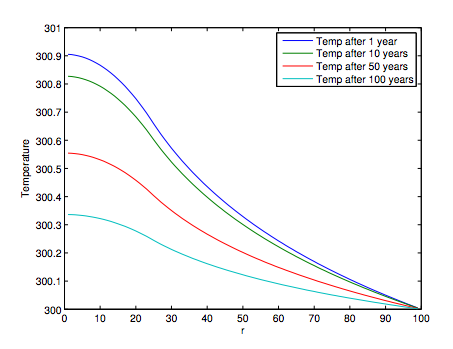
\includegraphics[width=100mm]{DrTemp.png}
\caption{Figure 5.3(b) from \cite{Olsen-Kettle} showing the temperature of the rod and its surroundings after different time periods.}
\label{DrTemp}
\end{figure}

Comparing the program output in \figref{Temp} to Dr. Olsen-Kettle's graph in \figref{DrTemp}, it is easy to see that the two methods produce nearly identical results. The discrepancy between the two graphs seems to show an increased temperature in the C code results, compared to the Matlab results. At its largest the difference is of the order of 0.05K (300.960 - 300. 905) at r = 1cm of the rod after 1 year (relative error on the order of $5\times10^{-5}$), the difference shrinks for the longer time periods and towards the radius edge such that they have the exact same value (300.0018) at r = 99 for the 100 year temperature.

This discrepancy could be due to the method of solving the matrix equation. The  gsl\_linalg\_solve\_tridiag, uses a form of Cholesky decomposition, whereas, Dr. Olsen-Kettle's MATLAB code uses the mldivide operator, which will analyse the matrix equation and decide which method is best to use to solve it. It can be seen from the mldivide site \cite{mldivide}, that it has a specific algorithm for tridiagonal matrices, but since the source code for mldivide is not available, one can only speculate as to which method the MATLAB code uses to solve tridiagonal matrix equations.

We can see which results are more likely to be accurate, through the use of a convergence test\cite{NumMethods}. This is a test where the step size is reduced, and it is expected that the answer does not change.

When the step size is reduced by a factor of 400 (m = 400,000) in an altered form of Dr. Olsen-Kettle's MATLAB code, the code runs for around 10 seconds, but the MATLAB results do not change significantly, and the graph looks exactly the same to the human eye.

When the step size is reduced by a factor of 400 in the C code, the code still runs in less than 5 seconds, however, the Temperature at r = 1cm after 1 year changes from 300.96 to 300.90, as shown in \figref{Tempred}, and larger reductions in step size even take this value below the convergent value found in Dr. Olsen-Kettle's results. This implies that the C code may not be convergent. Indeed, if the timestep is reduced by a factor of 1000 (m=1,000,000), this value at r=1cm for 1 year becomes 300.811K. 

\begin{figure}[htb]
\centering
\includegraphics[width=100mm]{Tempred.png}
\caption{The temperature of the rod and its surroundings after different time periods as produced by C code with a reduced timestep.}
\label{Tempred}
\end{figure}





\section{Conclusions}

This program can produce numerical or graphical results for the problem of a radioactive nuclear rod producing heat in a medium at any temperature.

The written C program is in fair agreement with the original MATLAB code and solution provided by Dr. Olsen-Kettle. However, the faster C code does not pass a convergence test, whereas the slower MATLAB code does, implying that the results of Dr. Olsen-Kettle are more reliable and more likely to be accurate.







\begin{thebibliography}{9}
\bibitem{Olsen-Kettle}
\url{http://espace.library.uq.edu.au/view/UQ:239427/Lectures_Book.pdf}
\bibitem{GSL}
\url{https://www.gnu.org/software/gsl/}
\bibitem{BEuler}
\url{https://en.wikipedia.org/wiki/Backward_Euler_method}
\bibitem{FiniteDifference}
\url{https://en.wikipedia.org/wiki/Finite_difference_method}
\bibitem{Linalg}
\url{https://www.gnu.org/software/gsl/manual/html_node/Tridiagonal-Systems.html#Tridiagonal-Systems}
\bibitem{mldivide}
\url{http://uk.mathworks.com/help/matlab/ref/mldivide.html;jsessionid=c331f174d51ef5ea5936761f6a38}
\bibitem{NumMethods}
\textit{Numerical Recipes in C, 2nd Edition (1992)}

\end{thebibliography}





\end{document}
